%======================================================================
\subsection{BW-MOD-16 --- Persistent section views (planned and built 25 Oct 2026)}\label{sec:mod16-plan}
%======================================================================

\begin{epic}{MOD-16}{Persistent section views}{M1}{\stDone}{(new, your request of 25 Oct; split from \eref{MOD-11})}
A section is a view you keep. It is saved in the file in a \emph{Sections} folder, the eye turns it on and off,
and a double-click edits it. Up to three planes cut at once. The cut faces are \emph{capped}: filled in each
part's colour, with a hatch that differs from part to part, and painted red where two parts' material overlaps on
the plane. Planes are moved and tilted with handles on the canvas or with fields in the right panel, and the fields
take expressions. The caps are drawn by the GPU with the stencil buffer, so no geometry is built and the view
stays live. The C++ node is taken from upstream PR~\#33186 and extended; the behaviour follows the Nxt add-on.
\emph{Acceptance:} on the Leonardo gearbox (\code{LE-02-01002}) a section through the axis caps all 24 components;
saved, closed and reopened, it is still there; stock FreeCAD opens the same file without a warning; three planes
cut at once; the old sun hub (rev.~1 of \code{LE-01-01009}) shows red on the cut where it meets the carrier; the
grid and datums are never cut; turning the model and dragging the plane stays above 30~frames a second.
\end{epic}

You asked on 25 Oct: ``can we fix the clipping so it works as a persistent section view like FreeCAD Nxt did''. The
section button on the navigation pill opens FreeCAD's \emph{Clipping} dock (\code{Std\_ToggleClipPlane},
\file{src/Gui/Clipping.cpp}). The dock cuts the view while it is open, forgets the cut when it closes, saves nothing
with the file and leaves the cut open: you look into the backs of faces (figure~\ref{fig:mod16-cuts}, left).
\textbf{A correction:} the Nxt review of 23 Oct (\S\ref{sec:uix-nxt}) listed the section view as ``already covered''.
It was not; this epic covers it. Your first answers:

\begin{center}
\small
\begin{tabularx}{\linewidth}{@{}lX@{}}
\toprule
Question & Answer (25 Oct)\\
\midrule
Engine & \textbf{Nxt's behaviour, drawn by C++ caps in the viewer}: the stencil node of upstream PR~\#33186 in our build,
  and the saved section objects in Python.\\
Where it lives & \textbf{Saved in the file, like a view} you turn on and off.\\
Planes and caps & \textbf{Up to 3} planes at once; caps \textbf{hatched}, a \textbf{clash in red}.\\
Interaction & \textbf{Handles on the canvas} (drag arrow, tilt rings) \textbf{and the right panel} (plane, offset and
  tilt as fields with expressions, Flip).\\
\bottomrule
\end{tabularx}
\end{center}

\begin{figure}[htbp]
\centering
\begin{subfigure}[b]{0.32\linewidth}\centering
  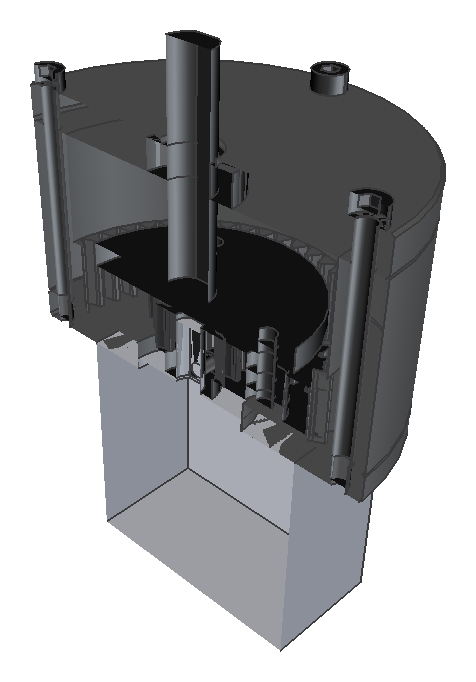
\includegraphics[height=6.4cm]{fig/mod16_today.png}
  \caption{Today: the Clipping dock's open cut. You see inside the parts.}
\end{subfigure}\hfill
\begin{subfigure}[b]{0.32\linewidth}\centering
  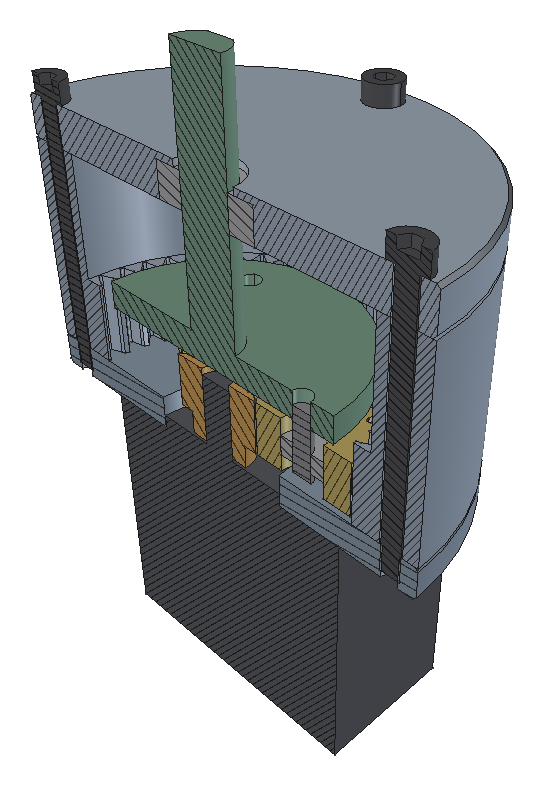
\includegraphics[height=6.4cm]{fig/mod16_target.png}
  \caption{The goal: every part capped in its colour, with its own hatch.}
\end{subfigure}\hfill
\begin{subfigure}[b]{0.32\linewidth}\centering
  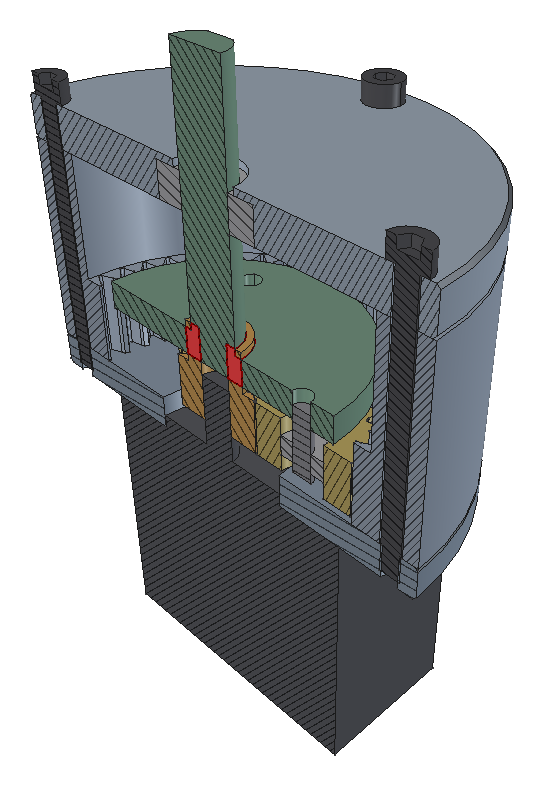
\includegraphics[height=6.4cm]{fig/mod16_clash.png}
  \caption{The old sun hub (rev.~1) meeting the carrier: 257.6\,mm\textsuperscript{3}, red on the cut.}
\end{subfigure}
\caption{The Leonardo gearbox (\code{LE-02-01002}) cut through its axis, rendered from a scratch copy on 25 Oct. (a)
is a real Coin clip plane. (b) and (c) are stand-ins built with exact Boolean cuts and a hatch laid over the cap faces
afterwards; the real caps are drawn on the GPU and need no Booleans. The red in (c) is the same clash the
interference check found on 24 Oct.}
\label{fig:mod16-cuts}
\end{figure}

%----------------------------------------------------------------------
\subsubsection*{1. What the spikes showed (25 Oct)}

Three scripts ran in a test FreeCAD 1.1.4 on a copy of your configuration, through the FreeCAD slot limiter, on a
scratch copy of the gearbox files (\file{section-plan/spike.py}, \file{spike2.py}, \file{target.py}). The vault was
only read, to fetch the old sun.

\begin{center}
\small
\begin{tabularx}{\linewidth}{@{}>{\hsize=0.75\hsize}X>{\hsize=1.25\hsize}X@{}}
\toprule
Check & Result\\
\midrule
Stencil buffer & FreeCAD asks for 8 stencil bits for every 3D view (\file{src/Gui/Application.cpp:2543}). The cap needs
  1 bit and the clash 1 more.\\
Coin clip planes & One, two and three \code{SoClipPlane} nodes at the top of the view's scene cut every part, links
  and assembly included, in 0.09\,s per offscreen frame. Placed there, they also cut the \textbf{grid}, so the real
  planes go below the grid, in front of the model only.\\
Several planes & OpenGL keeps a point only if it is on the kept side of \emph{every} plane, so two planes keep
  \emph{one} quarter. Fusion and SolidWorks remove one quarter and keep three (see the theory in~\S3 and
  question~1).\\
A section in the file & An \code{App::FeaturePython} \emph{Section} in a \emph{Sections} group keeps its plane, offset
  and on/off through save and reopen.\\
Without Heuretes FreeCAD & With its Python module missing, the same file opens and the object keeps its values; the Proxy is
  \code{None}, the recompute is clean and nothing is invalid. Stock FreeCAD just ignores it.\\
Upstream PR~\#33186 & ``Gui: hatched cross-sections for clipping planes'', open, review status \emph{changes
  requested}, last updated 18 Oct. 1\,145 lines in 14 files, all in \file{src/Gui}. It applies to our tree except one
  hunk of \file{View3DInventorViewer.cpp} (the includes). It adds \code{SoFCSectionCap}: per-part stencil caps for
  every active clip plane, each plane's cap clipped by the others, a stipple hatch per part, and the outline where the
  plane cuts. Transparent and open meshes are reported and left uncapped, and datums are never capped. It hooks into
  the Clipping dock and is not saved. In the review the author is narrowing it to one look, the part's own
  colour; reviewers asked for a hatch per part, quarter sections and a clash colour.\\
Nxt (\file{obelisk79/FreeCAD-Nxt}, LGPL-2.1) & \file{section\_object.py}: a \emph{Sections} group, at most three,
  saved, with the eye and double-click. \file{section\_view.py}, 1\,624 lines of Python: the same stencil method
  through raw OpenGL calls (\code{ctypes}), a hatch texture locked to the plane and snapped to the zoom, drag and tilt
  handles, the mouse wheel for the offset, and ``cut exactly'' into a Part feature. Its tracker reports the OpenGL
  loading failing on Windows (fixed 23 Oct): the fragility your C++ answer avoids.\\
\bottomrule
\end{tabularx}
\end{center}

%----------------------------------------------------------------------
\subsubsection*{2. How it will look}

\begin{figure}[htbp]
\centering
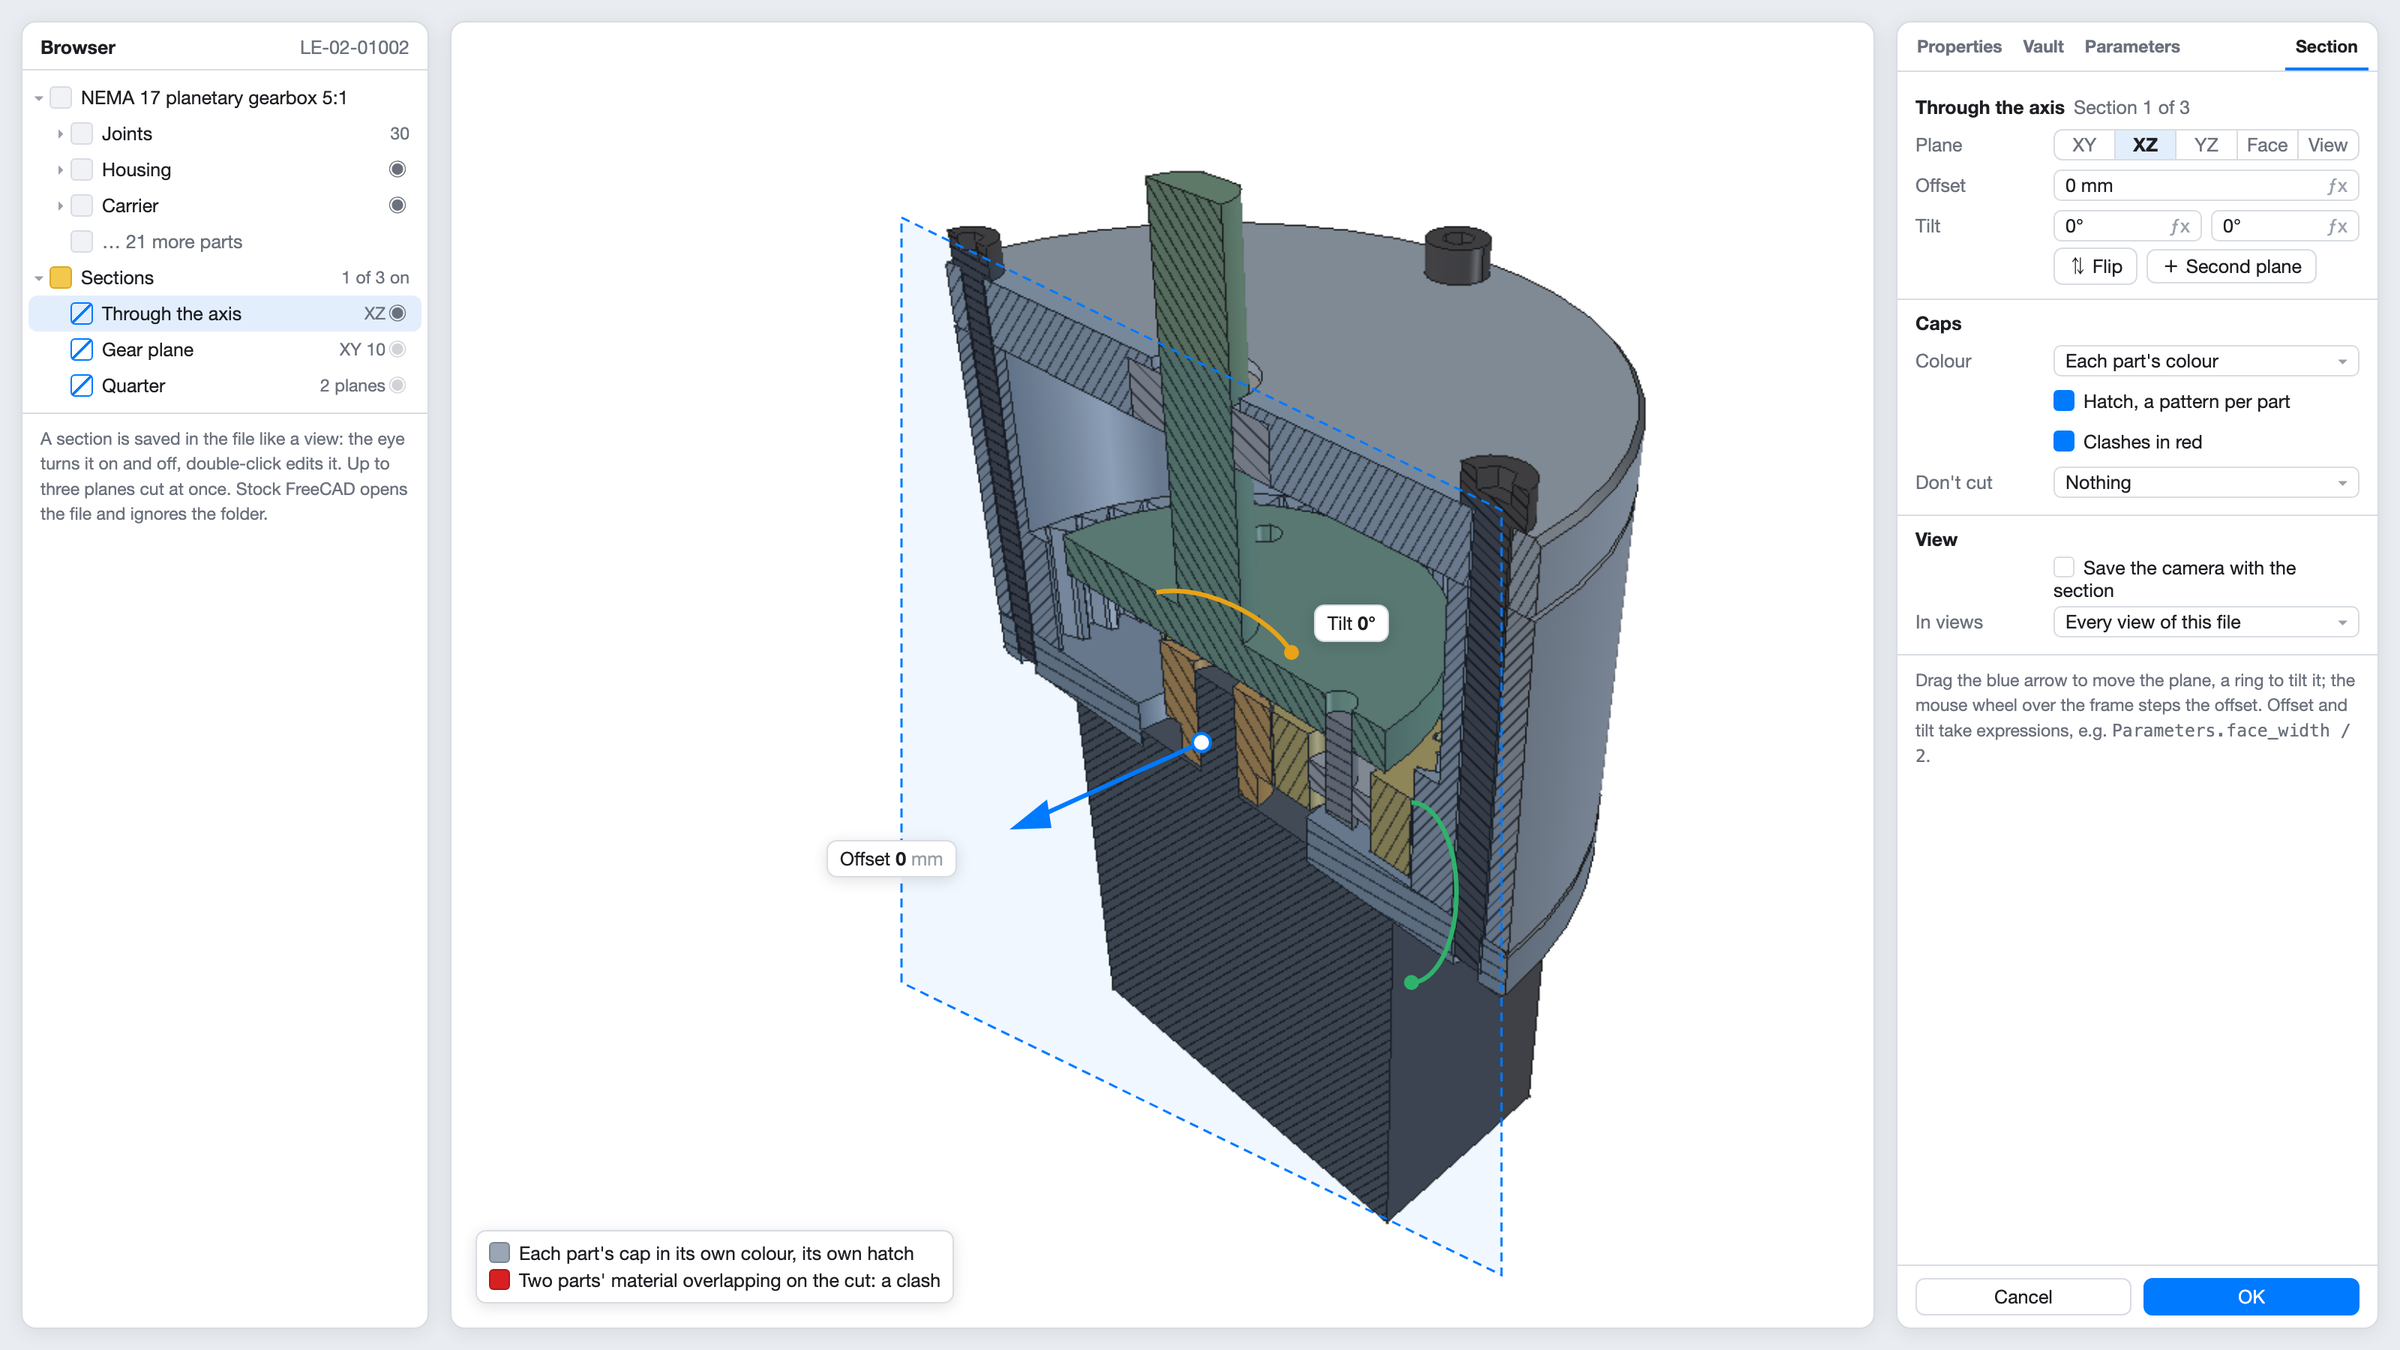
\includegraphics[width=\linewidth]{fig/mod16_mock.png}
\caption{Mock of the section view. Left: the \emph{Sections} folder in the Browser; one of three sections is on.
Middle: the section on the canvas, with the plane's frame, the blue drag arrow along its normal, two tilt rings
and the offset field. Right: the \emph{Section} command tab in the right panel (\eref{UIX-12}), open while the section
is edited. Plane, offset and tilt are on top, then the caps (colour, hatch, clash, parts not cut), then the view
options. The canvas image is figure~\ref{fig:mod16-cuts}(b).}
\label{fig:mod16-mock}
\end{figure}

%----------------------------------------------------------------------
\subsubsection*{3. Theory}

\paragraph{The clip plane.} A plane is a unit normal $\mathbf n$ and a distance $d$. A point $\mathbf p$ is kept
when $\mathbf n\cdot\mathbf p - d \ge 0$. The offset moves the plane along $\mathbf n$: $d = d_0 + s$. Tilting by
$\alpha$ about one in-plane axis $\mathbf u$ and by $\beta$ about the other, $\mathbf v = \mathbf n\times\mathbf u$,
turns the normal to $\mathbf n' = R_{\mathbf v}(\beta)\,R_{\mathbf u}(\alpha)\,\mathbf n$, about the point
$\mathbf c = d\,\mathbf n$ that stays put, so $d' = \mathbf n'\cdot\mathbf c$. \emph{Flip} is
$(\mathbf n, d)\mapsto(-\mathbf n,-d)$. With planes $1..k$ OpenGL keeps $\bigcap_i\{\mathbf n_i\cdot\mathbf p\ge
d_i\}$. A \emph{quarter section} that removes one corner and keeps three quarters needs the union instead,
$\{\mathbf n_1\cdot\mathbf p\ge d_1\}\cup\{\mathbf n_2\cdot\mathbf p\ge d_2\}$. That is two passes: draw the model
clipped by plane~1 alone, then again clipped by plane~2 and by plane~1 flipped, so the two passes never overlap. It
costs one more draw of the model while a quarter section is on.

\paragraph{Why the stencil finds the material.} Take a closed (watertight) part and a point $\mathbf q$ on the plane.
A ray from $\mathbf q$ to infinity crosses the part's surface an odd number of times exactly when $\mathbf q$ is
inside the part (the Jordan--Brouwer theorem). The eye's ray through a pixel meets the plane at such a $\mathbf q$.
Draw the part's triangles again, clipped by the plane, into the stencil only, with no depth test, and flip one bit
each time a triangle covers the pixel. The surface left after clipping lies on one side of the plane, so the bit
counts the crossings of the ray beyond $\mathbf q$:
\[
  \text{stencil}(x,y) \;=\; \Big(\textstyle\sum_{\text{triangles } t \text{ covering } (x,y)} 1\Big)\bmod 2
  \;=\; [\,\mathbf q(x,y)\in\text{part}\,].
\]
A quad on the plane is then drawn only where the bit is 1: that is the cap. The part's own depth decides what is in
front, so a cap hides behind nearer parts. Each part gets its own pass, which gives it its own colour and hatch. An
open mesh has no inside, which is why such a part is reported and left uncapped. With several planes, each plane's
cap is drawn clipped by the other planes, so a quarter section's two caps meet at the corner.

\begin{figure}[htbp]
\centering
\begin{tikzpicture}[scale=0.92, every node/.style={font=\small}]
  % left: parity
  \begin{scope}
    \fill[bwblue!8] (0,0) rectangle (6.2,3.6);
    \draw[thick, bwdark] (1.2,0.6) rectangle (5.0,3.0);
    \fill[bwgrey!25] (2.0,1.2) rectangle (4.2,2.4);
    \draw[thick, bwdark] (2.0,1.2) rectangle (4.2,2.4);
    \node[bwgrey] at (3.1,1.8) {hole};
    \draw[very thick, bwblue] (3.1,-0.2) -- (3.1,3.8) node[above] {plane};
    \fill[white, opacity=0.75] (0,0) rectangle (3.1,3.6);
    \node[bwgrey, align=center] at (1.5,3.3) {cut away};
    \foreach \y/\n/\c in {0.95/1/bwgreen, 1.8/2/bwred, 2.75/1/bwgreen} {
      \draw[-{Stealth}, \c, thick] (3.1,\y) -- (6.4,\y);
      \fill[\c] (3.1,\y) circle (2pt);
      \node[\c, anchor=west] at (6.45,\y) {\n\ crossing\ifnum\n>1 s\fi};
    }
    \node[align=center, font=\footnotesize] at (3.1,-0.65) {odd: material on the plane, so cap it;\\ even: the hole, so leave it};
  \end{scope}
  % right: clash
  \begin{scope}[xshift=9.6cm]
    \fill[bwgrey!20] (0,0.4) rectangle (3.0,3.0);
    \fill[bworange!35] (2.0,1.0) rectangle (4.8,3.4);
    \fill[bwred] (2.0,1.0) rectangle (3.0,3.0);
    \draw[thick] (0,0.4) rectangle (3.0,3.0); \draw[thick] (2.0,1.0) rectangle (4.8,3.4);
    \node at (0.9,1.0) {carrier};
    \node at (4.0,3.0) {sun};
    \node[white, font=\footnotesize\bfseries] at (2.5,2.0) {clash};
    \node[align=left, font=\footnotesize, anchor=north west] at (-0.2,-0.05) {bit 0: this part's parity (cleared per part)\\
      bit 1: ``a cap is already here'' (cleared per plane)\\ bit 0 $=1$ and bit 1 $=1$: red, else the part's cap};
  \end{scope}
\end{tikzpicture}
\caption{Left: the parity test on one part with a hole, seen edge-on. Rays from points on the plane run into the kept
half; an odd number of crossings means material. Right: two caps on the same plane. The carrier is drawn first and
sets bit~1. Where the sun's parity bit is also 1, its cap is drawn red.}
\label{fig:mod16-theory}
\end{figure}

\paragraph{The clash.} Two parts' caps on the same plane overlap where both parities are odd: the plane passes through
material of both, so their solids intersect there. A second stencil bit records it. It is cleared once per plane, and
every part's fill pass sets it with \code{glStencilOp(\dots, GL\_REPLACE)} on mask \code{0x2}. In a part's fill pass,
pixels where its parity bit is 1 and bit~1 is already set are drawn red (\code{glStencilFunc(GL\_EQUAL, 3, 0x3)}), the
others in its own colour (\code{GL\_EQUAL, 1, 0x3}). A section shows only the clashes its plane passes through; a clash
anywhere in the assembly is \eref{ASM-06}'s interference check. Parts meant to overlap, such as a screw in a tapped
hole (thread modelled at the tap-drill size), show red too. They can be marked \emph{fit} and left out, as in
question~7.

\paragraph{The hatch.} Each part's hatch is chosen from its name by the FNV-1a hash ($h \leftarrow (h\oplus b)\cdot
1099511628211 \bmod 2^{64}$ over its bytes), so a part keeps its hatch from session to session and neighbours differ.
PR~\#33186 draws the hatch as a 32$\times$32 \emph{screen} stipple: cheap, but fixed to the screen, so the lines do
not move with the part when you pan or turn the view. Nxt maps a hatch texture onto the plane, at a spacing $s$ in
model units that is snapped to the zoom, $s = 2^{\lceil\log_2(k\,w)\rceil}$ for $w$ model units per pixel. The lines
then stay on the part and keep about $k$ pixels apart at any zoom (question~2).

%----------------------------------------------------------------------
\subsubsection*{4. The design}

\paragraph{The saved section.} An \code{App::FeaturePython} named \emph{Section}, inside an
\code{App::DocumentObjectGroup} named \emph{Sections} at the root of the file. Its properties:

\begin{center}
\small
\begin{tabularx}{\linewidth}{@{}lX@{}}
\toprule
Property & Meaning\\
\midrule
\code{Plane} (\code{Placement}) & The plane: its local Z is the normal, its origin the point the tilt turns about.\\
\code{Mode} & \emph{XY, XZ, YZ, Face, View, Three points}: how \code{Plane} was made. \code{Support} (a link to the
  face or datum) keeps a Face section on its face when the part changes.\\
\code{Offset}, \code{TiltA}, \code{TiltB} & Distance and angles, each able to hold an expression (e.g.\
  \code{Parameters.face\_width / 2}).\\
\code{Flipped} & Which side is kept.\\
\code{Second} (optional) & A second plane for a quarter section, with its own offset and tilt; it counts towards
  the three planes.\\
\code{Caps}, \code{Hatch}, \code{ShowClash} & \emph{Part colour / one colour / none}; hatch on or off; clashes in
  red.\\
\code{NotCut} & Parts left whole (question~6).\\
\code{Camera} (optional) & The view saved with the section; turning it on goes there (question~5).\\
\code{Visibility} & The eye. At most three planes cut at once (question~9).\\
\bottomrule
\end{tabularx}
\end{center}

\paragraph{In the viewer (C++, \file{src/Gui}).} \code{SoFCSectionCap} comes from PR~\#33186 with its author's
copyright kept. It gains the clash bit, the hatch locked to the plane and the two-pass quarter section. A new
\code{View3DInventorViewer::setSectionPlanes()} puts up to three \code{SoClipPlane} nodes in front of the model only,
not the grid, the navigation cube or the draggers, and puts the cap node after the model. \code{View3DPy} exposes it
as \code{view.setSectionPlanes(planes, caps)}, and \code{view.sectionReport()} returns the per-part records (capped,
not cut, open mesh, transparent) for the panel and the tests. The Clipping dock keeps its own planes and works as
before (question~10).

\paragraph{In Heuretes FreeCAD (Python).} \file{bruceworx\_section.py}: the object and its view provider. Turning the eye on
sends the plane to every 3D view of the file, and turning it off takes it away. Recomputes, new views and switching
documents keep the views in step. Also in it: the commands \emph{New Section} (the navigation pill's section
button), \emph{Edit Section} (double-click) and \emph{Sections Off} (all at once), and the \emph{Section} tab in the
right panel (figure~\ref{fig:mod16-mock}). The handles are Coin draggers placed on the plane's frame: an arrow for
the offset, and two rings that snap to 5$^\circ$ with Shift for 1$^\circ$. The mouse wheel over the frame steps the
offset, Ctrl for a finer step. While one section is edited the others stay on, and the panel says
``2 of 3 planes in use''.

\paragraph{What is never cut or capped.} The grid, datums and origins (the PR already skips them), sketches,
annotation, and the joints' markers. Transparent parts and open meshes are cut but not capped, and the panel names
them: ``2 parts not capped: open mesh''.

%----------------------------------------------------------------------
\subsubsection*{5. Steps}

\begin{enumerate}[nosep]
  \item Bring PR~\#33186 into the fork (one include hunk to fix), build, and check it on the gearbox through the
        Clipping dock: every part capped, frame rate measured.
  \item \code{setSectionPlanes()} below the grid; the clash bit; the plane-locked hatch; the quarter section's two
        passes; \code{sectionReport()}.
  \item The Section object, its view provider, the three-plane limit, save and reopen, and stock FreeCAD opening the
        file.
  \item The Section tab with expressions, then the handles and the mouse wheel.
  \item The navigation pill's section button and the commands; the context menu in the Browser.
  \item Tests. Unit: plane, tilt and flip arithmetic, and the save round-trip. Viewer: \code{sectionReport()} says
        ``capped'' for all 24 gearbox components; an offscreen render of two overlapping boxes has red pixels exactly
        in their overlap and none without it; the grid is uncut. A narrated GUI test in a left-half test window.
  \item Report the clash bit and the plane-locked hatch to the PR's author as a follow-up (question~11).
\end{enumerate}

%----------------------------------------------------------------------
\subsubsection*{Questions (answered 25 Oct: all thirteen recommendations)}

\begin{enumerate}
  \item \textbf{Quarter section.} When a section has two planes, remove one corner and keep three quarters (Fusion,
        SolidWorks; one more draw of the model), or keep one quarter (what OpenGL does by itself)?\\
        \emph{Recommendation:} remove one corner; that is what you expect from a quarter section.
  \item \textbf{The hatch.} Locked to the plane, so it moves with the part and stays a few pixels apart at any zoom
        (Nxt), or fixed to the screen (the PR, simpler)?\\
        \emph{Recommendation:} locked to the plane; it reads like a drawing and does not swim when you turn the view.
  \item \textbf{The default look.} Each part's colour with its hatch (the mock), or one grey for every cap, as one
        reviewer of the PR prefers? Both stay as options.\\
        \emph{Recommendation:} each part's colour and hatch; on the gearbox it tells the carrier from the sun at a
        glance.
  \item \textbf{Clash list.} Besides the red on the cut, list the pairs that clash on the plane in the panel (``Sun /
        Carrier''), with a \emph{Measure} button for the exact volume?\\
        \emph{Recommendation:} yes. The list comes from the caps and costs nothing; the volume is measured only when
        you ask.
  \item \textbf{``Like a view''.} Should a section also save the camera, so turning it on swings the view to where it
        was made?\\
        \emph{Recommendation:} an option per section, off by default; turning a section on should not move your view
        unasked.
  \item \textbf{Parts not cut.} Drawings leave shafts, pins, screws and keys uncut along their length. Offer \emph{Don't
        cut fasteners and pins} (by the part's \emph{Item type}, COTS hardware), as well as picking parts by hand?\\
        \emph{Recommendation:} both, off by default.
  \item \textbf{Intended overlaps.} A screw modelled at its full diameter in a tap-drill hole clashes by design. Mark
        such pairs as \emph{fit} (saved with the section) so they are not red, or leave them red?\\
        \emph{Recommendation:} let a pair be marked \emph{fit} from the clash list; it is remembered per file.
  \item \textbf{Where in the Browser.} A \emph{Sections} folder at the root of the file, or under the assembly?\\
        \emph{Recommendation:} at the root; a part file has sections too, and the folder stays out of the BOM.
  \item \textbf{A fourth plane.} With three planes in use, turning on another section: refuse with a message, or turn
        off the one used longest ago?\\
        \emph{Recommendation:} turn off the oldest and say so in a toast with \emph{Undo} (\eref{UIX-10}).
  \item \textbf{The Clipping dock.} Keep it under \emph{View} as it is, with the navigation pill's section button
        going to sections, or remove it?\\
        \emph{Recommendation:} keep it; nothing else changes for people who use it.
  \item \textbf{Upstream.} Offer the clash bit and the plane-locked hatch to PR~\#33186's author once they work
        here?\\
        \emph{Recommendation:} yes, as a follow-up PR on top of theirs. It keeps our C++ close to what upstream may
        merge.
  \item \textbf{Exact cut.} Also offer Nxt's \emph{Make a solid from the section} (a Part feature, for printing or a
        drawing)?\\
        \emph{Recommendation:} not now. Section views on drawings are TechDraw's job (\eref{DRW-06}).
  \item \textbf{Which views.} A section that is on cuts every 3D view of the file, or only the view it was turned on
        in?\\
        \emph{Recommendation:} every view of the file, as the mock says; a second view of the same part then shows
        the same section.
\end{enumerate}

%----------------------------------------------------------------------
\subsubsection*{6. Built (25 Oct)}

Built the same day on your answers. What runs:

\begin{center}
\small
\begin{tabularx}{\linewidth}{@{}>{\hsize=0.7\hsize}X>{\hsize=1.3\hsize}X@{}}
\toprule
Piece & What it is\\
\midrule
C++ caps & \file{src/Gui/Inventor/SoFCSectionCap.cpp} from PR~\#33186, with the stencil re-laid out: parity in bit~7, the
  id of the part already capped in bits~0--6. Over 0x80 is a clash. Clash pixels per pair are counted with an occlusion
  query, measured with the colour off first, so overlaps under 12~px are capped as usual. Hatch texture locked to the
  plane, snapped to the zoom. Seams. Parts left whole. Caps lifted towards light grey (35\,\%) so dark parts read.\\
Viewer & \code{View3DInventorViewer::setSectionPasses} puts one separator per pass (clip planes, \code{objectGroup}, the
  caps) in \code{objectGroup}'s place, so only the model is cut. \code{View3DPy}: \code{setSectionPasses},
  \code{clearSectionPasses}, \code{getSectionReport}. Offscreen renders and thumbnails now get a stencil buffer
  (the FBOs were depth-only).\\
A Coin bug & Coin 4.0.3, our build's, crashes when a \code{SoCallbackAction} with per-type callbacks is destroyed
  (\code{deleteAll()} on empty slots, fixed in coin3d 4.0.4). PR~\#33186 crashed on it at once. Worked around by a no-op
  callback for every node type.\\
Heuretes FreeCAD & \file{bruceworx\_section.py}: the Section object and the Sections folder, the three-plane limit with an Undo
  toast, the Section tab (expressions, Flip, quarter, caps, the clash list with \emph{Mark as fit} and \emph{Measure},
  the saved camera), the handles (blue arrow out of the cut, orange and green tilt rings, drawn over the model), the
  commands \emph{Section View} (the navigation pill's button and the View menu) and \emph{Sections Off}.\\
\bottomrule
\end{tabularx}
\end{center}

\emph{Different from the plan:} datums, sketches and joint markers that belong to a part are cut with it. They share its
branch of the scene, and Coin clips by branch. The grid, measurements and overlays are never cut. \emph{Don't cut
purchased parts} reads the part property \code{ItemType = cots}: none of the gearbox's COTS parts has it set yet, which is
a vault data fix for you to approve.

\emph{Checked:} 16 unit tests (plane arithmetic, passes, the limit, save and reopen, COTS through links) and a narrated
GUI test on a copy of the gearbox:
\begin{itemize}[nosep]
  \item the section caps every part it cuts, at 89--93~frames a second while turning;
  \item Mark as fit takes M3$\times$40-in-the-plate out of the red;
  \item typed offsets, the quarter section and save and reopen all work, and a fourth section turns the oldest off;
  \item parts left whole are drawn whole;
  \item the old sun hub shows Sun/Carrier at 2\,980~px, and Measure gives 257.6\,mm\textsuperscript{3};
  \item the handles move the offset and step the tilt by 5$^\circ$, and Cancel undoes both.
\end{itemize}

\begin{figure}[htbp]
\centering
\begin{subfigure}[b]{0.24\linewidth}\centering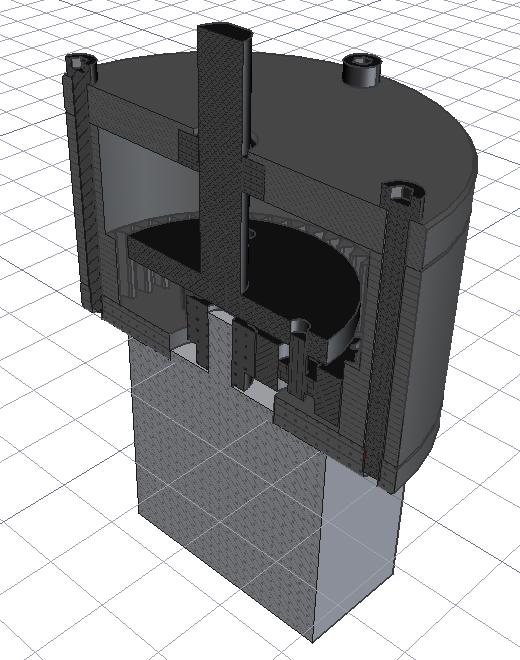
\includegraphics[width=\linewidth]{fig/mod16_built_half.png}\caption{Half section}\end{subfigure}\hfill
\begin{subfigure}[b]{0.24\linewidth}\centering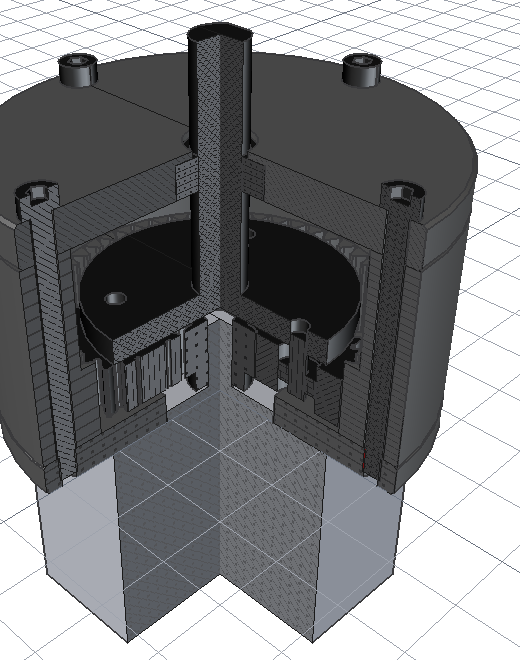
\includegraphics[width=\linewidth]{fig/mod16_built_quarter.png}\caption{Quarter section}\end{subfigure}\hfill
\begin{subfigure}[b]{0.24\linewidth}\centering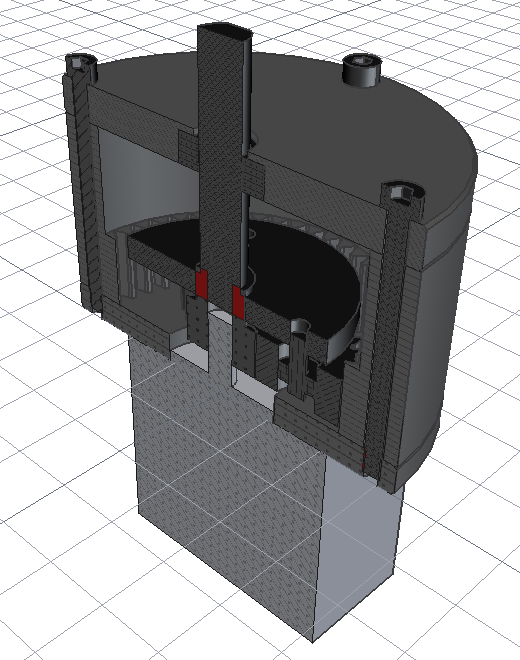
\includegraphics[width=\linewidth]{fig/mod16_built_clash.png}\caption{Old sun hub: red}\end{subfigure}\hfill
\begin{subfigure}[b]{0.24\linewidth}\centering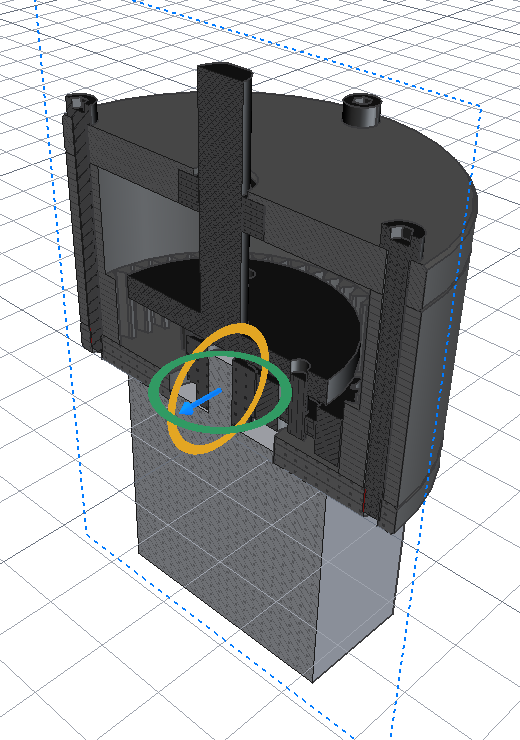
\includegraphics[width=\linewidth]{fig/mod16_built_handles.png}\caption{Editing: the handles}\end{subfigure}
\caption{The built section view on a copy of the gearbox, rendered by the viewer itself (offscreen, so with the
stencil buffer now given to offscreen renders). The grid is uncut.}
\label{fig:mod16-built}
\end{figure}
